%%%%%%%%%%%%%%%%%%%%%%%%%%%%%%%%%%%%%%%%%%%%%%%%%%%%%%%%%%%%%%%%%%%%%%%%
\section{Profiling}
\label{sec:profiling}
%%%%%%%%%%%%%%%%%%%%%%%%%%%%%%%%%%%%%%%%%%%%%%%%%%%%%%%%%%%%%%%%%%%%%%%%

\begin{figure*}[t]
  \begin{center}
    \subfloat[The out on SSD (identical for YOLO): initialization phase, followed by serial object detection of images]{
      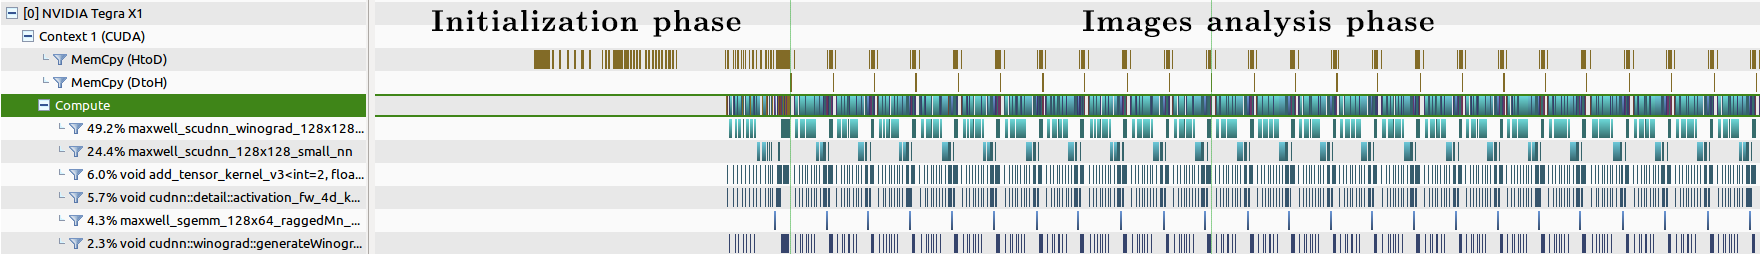
\includegraphics[width=1\textwidth]{./imgs/ssd-10frames.png}
      \label{fig:profile:ssd_full}
    } \\
    \subfloat[Zoom in on SSD: single image object detection]{
      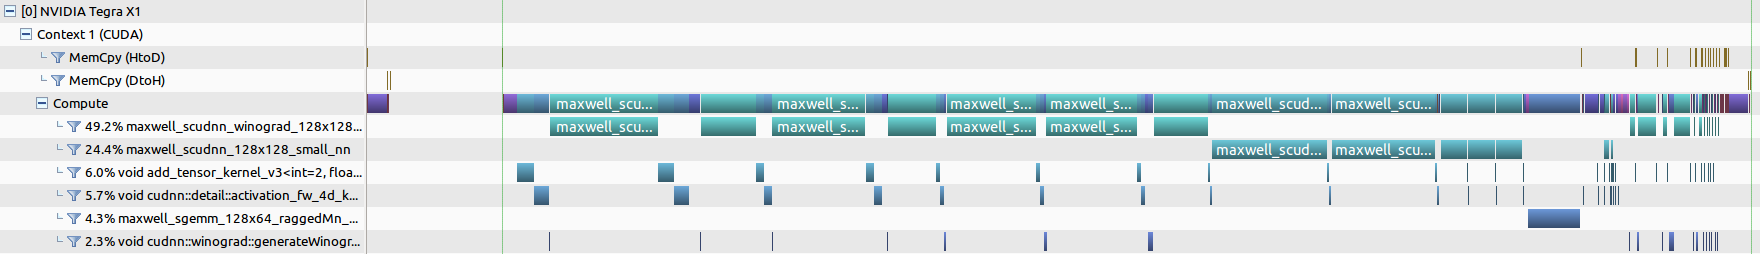
\includegraphics[width=1\textwidth]{./imgs/ssd-1frame.png}
      \label{fig:profile:ssd}
    } \\
    \subfloat[Zoom in on YOLO: single image object detection]{
      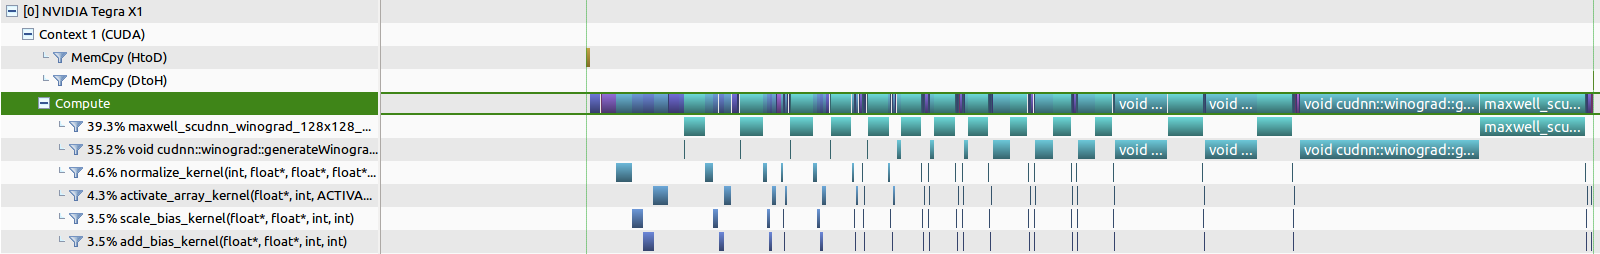
\includegraphics[width=1\textwidth]{./imgs/yolo-1frame.png}
      \label{fig:profile:yolo}
    }
    \caption{Profiling object detection on a batch of images with GPU and cuDNN on Jetson TX1, using NVIDIA Visual Profiler}
    \label{fig:profile}
  \end{center}
\end{figure*}

Figure \ref{fig:profile} shows the profiling output of object detection for a batch of images, using SSD and YOLO. Profiling was done using NVIDIA Visual Profiler.

One of Jetson's strengths is that its CPU and GPU share the same memory. Therefore, host-to-device (HtoD) and device-to-host (DtoH) copies can be optimized to zero-copy \cite{tegrazerocopy}. Zero-copy will have no effect on SSD and YOLO, since memory copies are not frequent, therefore, there is no speedup potential. In addition, there are no overlapping opportunities between HtoD, DtoH, and the compute kernels, since there are almost no memory copies.

There is no parallelism between kernels. SSD and YOLO fetch and analyze each image in serial, so theoretically, one can analyze a couple of images in parallel. However, Jetson TX1 has only 2 SMs, with 128 CUDA cores each, therefore, adding additional threads to the system, or running two or more object detection processes in parallel, achieves no performance gains. Since SSD is implemented in Caffe as a series of layers, a possible solution may be to combine layers and avoid unwanted syncing that prevent kernel concurrency.

As can be seen from the profiling output, the dominant computation kernels belong to the cuDNN library. Both SSD and YOLO use cuDNN computations more than 70\% of the total computation time. This implementation is given, and cannot be changed by the user of the library. Therefore, the computation time cannot be improved significantly.

A major difference between SSD and YOLO, is number of memory transfers per frame. While YOLO has a single DtoH transfer and a single HtoD, SSD has 32 DtoH transfers and 2 HtoD transfers. Most of the SSD DtoH transfers are 16 bytes in size; very small and inefficient transfers. We did not manage to isolate the SSD Caffe layers that cause this issue.  



